\documentclass[12pt]{scrartcl}

\usepackage[english]{babel}
\usepackage{tuebingerspruechle}
\usepackage{qtree}
\usepackage{aleks}
\usepackage[utf8x]{inputenc}
\usepackage{linguex,natbib,graphicx}

\author{Aleksandar Dimitrov}
\title{Rebuilding WERTi: Providing a Platform
for Second Language Acquisition Assistance}

\bibliographystyle{plainnat}

\begin{document}
\maketitle

\tableofcontents

\SpruechleAufsagen{Aleksandar Dimitrov}

\section{Introduction}

Using tools and methods made available through recent achievements in computational
linguistics and related subjects to ease the process of second language
acquisition has only recently gained focus in research projects.  While
digitalized versions of traditional data sources like dictionaries have already
experienced usage to some extent, we have yet to discover new and
effective ways of aiding second language acquisition of adult learners. Many
systems have so far been proposed and their implementations vary in quality and
focus.

WERTi tries to approach this problem from a general perspective. Making
use of the momentum of the Internet, WERTi provides a platform for
implementing linguistic analysis and subsequent input enhancement methods on
user specified pages from the World Wide Web. Using Java Servlet and AJAX technology for
serving content and the UIMA framework for processing it in a dynamic and
flexible manner, the goal is to provide a platform for linguistic processing of
online content that can go beyond input enhancement and engage new and
interactive methods.


\subsection{Concept \& Design}

The original design of WERTi has been developed at Ohio State University by
\textsc{Detmar Meurers}, \textsc{Vanessa Metcalf}, \textsc{Luiz Amaral},
\textsc{Chris Kovach} and \textsc{Cory Shain}.
It is accessible at the following internet address:

\ex. \texttt{http://prospero.ling.ohio-state.edu/WERTi}

The underlying research on WERTi is best summarized in \cite{talk1} and \cite{talk2}.

At Tübingen University the concept has now been extended to encompass a wider
range of functionality and provide a more scalable solution. To achieve this,
several enterprise grade technologies have been put to use. Although this comes
with certain drawbacks (such as an increase in the code base by as much as over
1000\%), they provided the developer with a more flexible and robust architecture which
should be able to cope with most demands to the system. The development of the
new system started on May 8th in 2008 and has been going on for one and a half month
as of writing this paper.\footnote{Acknowledgements:
I would like to thank my advisor \textsc{Detmar Meurers} for providing
the unique opportunity on working on the WERTi system. 
I would also like to thank \textsc{Janina Radó}, who provided invaluable feedback
about the writing of academic papers and also suggested some features for the
system.}
 In this time, a total of over 3300 lines of Java code
 have been written\footnote{And countless more have been rewritten}, accompanied by about 2000 lines of XML code, mainly in the
descriptor files for UIMA and the interface models.  Additionally, about 5000
lines of documentation in HTML have been generated by the system and the
developer. All of the development progress has been kept track of in a version
control system, so historical changes are easy to
comprehend.
\section{The Development Process}

This section first explains the goals of the reimplementation and then
displays in what environment the project has been written and what technologies
have been put to use.

\subsection{Goals of the New Implementation}

 While the original implementation was
 written in the programming language
 Python, the new design is rooted in Java
 technologies and makes use of several frameworks to ensure maximum scalability.
 
The new system was written with several aspects in mind:
\begin{itemize}
  \item While the original system was restricted to a few hand picked web sites
    and in fact only supporting input from one particular news
    site\footnote{This site was \texttt{http://www.reuters.com}}, the new system
    should be able to support almost arbitrary input from sites in the World
    Wide Web. For this the system has to perform reliable and robust evaluation
    of the site content in order filter out text for later natural language
    processing tasks. This way the system can provide the user with free choice over the
    target material %% YAY!
  \item Processing of site content was to  be generalized and made to be as
    flexible as possible in order to ensure maximum extensibility of the
    system. This also implied splitting up different parts of natural
    language 
    processing tasks on the input into several interdependent steps. This way,
    the results of one of the \emph{Analysis Engines} can always serve as the
    input to other engines. Using UIMA, all processing can happen at a
    meta-level through annotations, while leaving the document text stateless
    and thus ensuring consistency among processing steps.
  \item Asynchronous client $\leftrightarrow$ server communication capabilities
    were to be ensured in
    order to allow evaluation of the user's performance on target texts.
    Together with an anticipated user account system this would provide
    the ability of measuring of a particular user's progress and provide them
    with automated feedback on their abilities.
  \item Overall the goal was to provide an easy to use, flexible and scalable web 
    based platform for methods of second
    language acquisition assistance.
\end{itemize}

\subsection{Design Process} The work on the Java implementation of WERTi 
was mostly conducted by one person. Given free choice over the
development environment and frameworks, a considerable part of the writing
process was spent on evaluation and study of the technologies to be applied. The
only notable specifications set on the development environment were the use of
UIMA, which in turn implied the use of the Java programming language.

Development happened in a very productive atmosphere with mostly weekly project
meetings between the programmer and the project supervisor where core
functionality and the design of the analysis process were discussed. During the
course of the design process, the system was several times restructured and some
parts of it have by now been completely rewritten two or even three times.

Work on the code has to a great extent been  performed using standard UNIX command line
tools for writing, testing and debugging code. More advanced solutions
like the Eclipse Java IDE were also used because of their capabilities which
allowed for organization of the work within the different frameworks in a more
straight-forward way\footnote{Most
importantly UIMA which comes with a number of useful Eclipse plug-ins to easily devise
analysis engine descriptors.}. All of the work has been tracked with a version
control\footnote{The author chose to use the \emph{git} version control system,
which has been and developed for and successfully used in the context of much greater
code bases, such as the Linux kernel.} system on which further work on the system
will also depend.

\section{The Architecture of the System}

This section will explain the principles underlying WERTi's functionality by
first looking at the data processing architecture and then showing how it is
integrated into the user interface of the web application.


\subsection{The UIMA Analysis Engines}\label{sec:UIMA}

All text extraction and natural language processing work is done inside the UIMA
architecture.  Modifications  to the document's structure are clearly separated
from the process of annotating it. This allows for ensuring natural language
analysis is a consistent process on one static input document.

The NLP routines only add annotations to the document, and they are not supposed
to change its state in any other way. Enriching the content of the web site is
then left to an outside module that processes only the annotations and does not
look at the document text itself. To achieve this degree of encapsulation
between the different tasks, the system has been split into three main parts,
operating independently:

\begin{itemize}

\item{ HTML processing (Pre-Processing): } 

  During initial processing of the input text, which at this stage consists of
  the raw web site content retrieved by the server,  HTML tag annotations are
  made to distinguish HTML tags as non-natural language text. Then another
  module finds ``relevant'' text within the text surrounded by tags. This lays
  ground to later linguistic analysis by setting the margins of which parts of
  the document it has to operate on.

\item{ Linguistic Processing: } 
  
  All linguistic tasks (tokenization, sentence boundary detection,
  part-of-speech tagging\ldots{}) on the text-annotations from the previous
  processing step are performed in this module. This is also the most expensive
  step from a computational point of view. Optimizations to the code are most
  likely to yield visible results here.

\item{ Enhancement Processing (Post-Processing): }
  
  Post processing analysis provides annotations on the document text with regard
  to the enhancement method the user inquired.  \end{itemize}

All steps operate solely on the CAS, UIMA's native document model. This is also
the most strenuous requirement on analysis engines to be integrated into WERTi.
While external configuration may be read, there should be absolutely no side
effects outside the CAS - which is the only stateful entity during
linguistic processing.

The next sections will explain all subsequent analysis steps in further detail.

\subsection{HTML Processing}

The HTML processor method was designed to be primitive and efficient. While
using a fully capable HTML parser was considered, a more simple approach was
favored over a fully markup-aware and more heavy parsing.
Full and formally correct HTML markup was deemed unnecessary and
parsing too time intensive and error-prone.
Furthermore, changing the
implementation of an analysis step even this fundamental to further processing
should be easy and without side-effects as long as the requirements to
preconditions and postconditions are met.

\paragraph{Preconditions} An input document retrieved in during earlier steps
has been retrieved and it exists in memory as an instance of a singleton
String\footnote{As usual in UIMA. For large documents, UMIA provides ways of
splitting up documents and processing the chunks independently. However, UIMA
only considers documents well beyond one megabyte to be ``big enough'' to be
split. The plain HTML most web pages serve rarely exceeds this mark.}   and is
stored in the UIMA CAS.
\paragraph{Postconditions} The document contains annotations marking up the
positions and spans of HTML tags in the document text. The names of
tags\footnote{E.g. ``p'' for the tag \texttt{<p>} or ``div'' for the dag
\texttt{<div>}.} are
also stored and a flag is set that denotes whether this tag is
closing another sibling\footnote{A preceding slash in the tag name closes the tag.}.

\subsection{Finding Text to Process}

The next step in the pipeline is to find a way of denoting the text areas that
will lay the basis for later linguistic processing. Originally this part of the
analysis engine was far more productive than it is now. It has lost a large part of its
functionality which has been taken over by the linguistic processing
itself.\footnote{Coherence analysis during sentence boundary detection, which is
explained further on has replaced a more specialized approach of trying to find
bits of natural language that do not constitute a full text (e.g. choices in a
menu or short statements in tables.)}

Currently, its main task is to eliminate whitespace and text between tag pairs
considered irrelevant, mostly because they contain scripts and meta-information
not actually rendered to text by the user's client.

This functionality could be further extended by providing hints and special
cases for certain recommended web sites, such as Wikipedia or various news
sites. However, since the source layout of most web pages is highly volatile,
development focus has so far not turned to evaluation of this idea.

\paragraph{Preconditions} The CAS contains full HTML tag annotations.
\paragraph{Postconditions} The CAS contains a markup of all text that is going
to be considered by the linguistic processing.

\subsection{Linguistic Processing}

Linguistic processing currently goes through 3 major steps: \emph{Tokenization},
\emph{Sentence Boundary Detection} and \emph{Part of Speech Tagging}. This
steps subsequently depend on each other.

\subsubsection{Tokenization}

Tokenization chunks the input from the previous processing steps into tokens of
natural language. Different tokenizers may perform differently and consider
different type of input spans to denote ``tokens''. Taking this into account is especially important
since later steps may depend on a particular type of tokenization 
rules\footnote{Part of speech tagging is particularly sensitive to
tokenization. Penn Tree Bank trained taggers usually require tokenization to
happen according to the PTB tokenization guidelines. Currently, WERTi's
tokenizers respect this guidelines, to provide a most general rule processing can
rely on.}. Several tokenizer engines have been implemented, with the current
alternatives being an interface to the Stanford Tagger's
tokenizer\footnote{This tokenizer was written by \textsc{Tim Grow}, \textsc{Teg
Grenager}, \textsc{Christopher Manning}, \textsc{Jenny Finkel}} 
and a simple example tokenizer, implemented locally for testing purposes, which
seems to perform similar in terms of quality, but better in terms of performance
and is the current default.

\paragraph{Precondition} The CAS contains annotations that denote possible input to
linguistic processing tasks.
\paragraph{Postcondition} The CAS contains a set of token annotations that can lay 
ground to all further linguistic analysis.

\subsubsection{Sentence Boundary Detection}

The sentence boundary detector implemented is currently not very advanced and
simply matches several regular expressions and even single characters considered
to end a sentence in all cases (\verb#.#, \verb#?# and \verb#!#). This could be
improved by making more educated assumptions about the nature of the input
tokens, but development has not focussed on these issues so far. While part of speech
tagging does generally benefit from stringent denotations of sentences, the
tagging process has so far been accurate enough and 
providing a correct method of sentence boundary detection could prove
non-trivial to implement. This could also be an entry point for future projects
to improve the system's functionality, as accurate sentence boundary detection
is of great importance to syntactic parsing.

This step also analyzes the denoted sentence's \emph{coherence}. This means, it
takes a simple statistical measure into account that compares the volume of text
against the number and length of tags over the sentence's span in the raw
document text. This has proven to be useful in avoiding ``enhancement'' of user
interfaces of web pages and other elements not desirable as targets for input
enhancement.

\paragraph{Precondition} Annotations in the CAS exist for all relevant input
tokens in natural language.
\paragraph{Postcondition} The CAS contains a markup of sentence boundaries. This
markup only depends on a starting and an ending point within the document text,
possibly spanning HTML tags\footnote{UIMA provides a \texttt{subiterator} method to
construct an iterator over annotations of a particular type that are subsumed by
another annotation of arbitrary type. It does not provide a general mechanism
for implementing distributed annotations that would have multiple beginning and
ending points.}. The sentence annotations also contain coherence values between
0 and 1, with 1 denoting maximum coherence (only text tokens and no tags) and 0
denoting minimum coherence.

\subsubsection{Part of Speech Tagging}

Part of Speech tagging currently relies solely on external tools. Two taggers
have so far been implemented: The \emph{Penn Tree Bank Tagger}\footnote{Written
by \textsc{Kristina Toutanova}, \textsc{Miler Lee}, \textsc{Joseph Smarr},
\textsc{Anna Rafferty}} and the
\emph{UIMA Sandbox Tagger}. A Java \emph{Interface} in the analysis package
provides a common abstraction mechanism over the different taggers to be
implemented. The \verb#Tagger# interface declares processing methods as
\verb#synchronized#, so calls to the tagging routines are blocking. This ensures
multiple clients running on the same server will not hinder the tagger in
processing each call correctly\footnote{No tagger of those evaluated for usage
provides concurrent processing of input strings since tagging is generally
deemed to be an expensive step the machine performing it should focus on.}.

Taggers are stored statically in server side context to ensure maximum
performance as tagger instantiation is typically very costly. Most taggers
are stateless during tagging, ensuring equal quality of results among calls.

Taking into account sentence coherence a explained earlier is not enforced, but
encouraged.

\paragraph{Precondition} The CAS contains annotations denoting tokens of natural
language and sentences thereof. The tagging process feeds on two types of annotations:
\verb'Token's and \verb'Sentence's. It has access to the token annotations via
calls to the sentence annotation's subiterator.

\paragraph{Postcondition} All \verb'Token' annotations the tagger found tags for
now carry a ``tag'' field, indicating their part of speech tag. The annotator
engine does not create new tag annotations, but retains a semantic relationship
between tokens and their part of speech tags by using an annotation field to
store the tag in.

\subsubsection{Post Processing - Input Enhancement}

This step depends on
  annotation results from the two preceding modules; certain HTML markups are
  used in order to correctly organize all code later executed on client side.
  While this is the last step performed by the analysis engines, it is still
  non-destructive with respect to the document text as it only marks entry
  points for enhancement code. Every annotation contains a list of document
  positions and a corresponding list of enhancement strings to be put into the
  respective document positions. Each enhancement also covers a certain span -
  this way the enhancement process which generates the final HTML page to be
  returned to the user can make sure enhancements don't overlap or conflict.

  \paragraph{Precondition} There exist annotations in the CAS which can be used
  as anchor points for enhancements. Different post processing modules will
  depend on different kinds of annotations. The current \verb#PoSEnhancer#
  depends on \verb#Token# annotations which carry information about their
  part of speech tags.
  \paragraph{Postcondition} The CAS contains enhancement annotations the main
  system can use to enhance the document.

\subsection{The User Interface}

At the time of writing the user interface to the WERTi platform has not been
finished yet. As such, this section mostly provides a perspective on desired
functionality, indicating partial results when they are already implemented.

\subsubsection{The Interactive Web Interface}

WERTi is now a web application, written in the Google Web Toolkit, which
compiles native AJAX code from Java sources. The toolkit thus provided a
possibility of increasing the consistency of the platform's code by ensuring
that it would be written using only one programming language. The user interface
components rely on RPCs to interact with the server. RPCs\footnote{Remote
Procedure Calls} provide an asynchronous method of interaction between client
server side code, so the user can be informed about the progress of their
request and also interact seamlessly with generated enhancements. While basic
proof of concept for the user interface is already finished, more components
will be implemented shortly. Some of the functionality intended for the system
includes:
\begin{itemize}
  \item Users should be provided with an account system and components for
    evaluating their own progress in certain parts. For this, a basic database
    interface has been written, connected to the PostgreSQL engine. Calls to the
    database will be implemented in an asynchronous fashion, making use of
    non-blocking threading on the server side.
  \item Input enhancement on the retrieved document should make more use of its
    potential brought by the underlying framework. The chosen methods would
    allow for interactive suggestions and on line feedback, as well as the
    implementation of interesting new features possibly relying on client/server
    interaction. Partial translation of the document text or only dictionary
    lookups would be one such feature.
\end{itemize}

The main reason for the user interface to be in a usable, but yet to be finished
state is that development focus laid on making the back end reliable and stable
enough to deal with user requests first. With a solid base provided, the user
interface can now make use of the functionality described earlier in section
\ref{sec:UIMA}.

\subsection{Summary: A General Overview}

A bird's eye view of the system's architecture is provided in \ref{digraph}.

\begin{figure}[htp]\label{digraph}
  \centering
  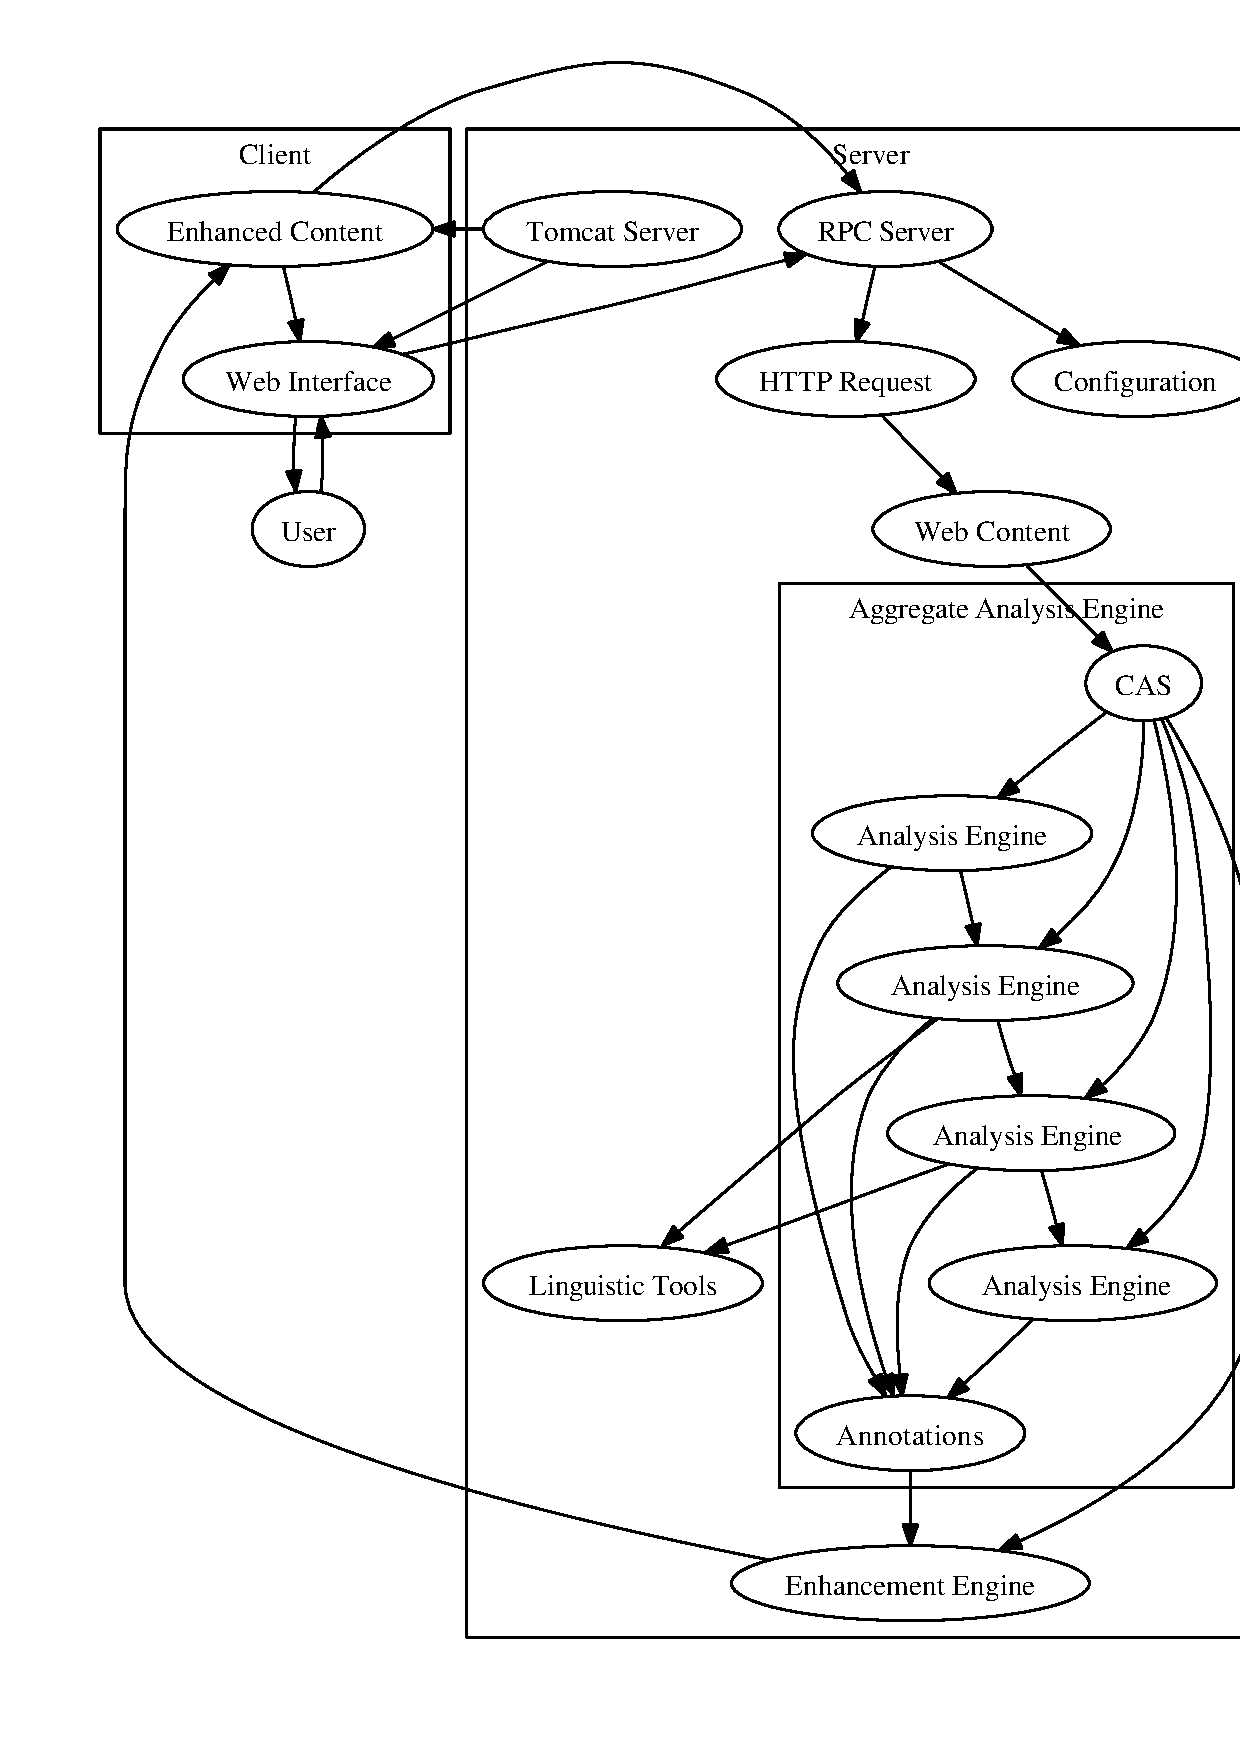
\includegraphics[scale=0.45,angle=90]{architecture}
  \caption{A simple overview of WERTi's current architecture}
\end{figure}

Here the arrows denote general a communication pipeline between two components. The
graph shows how the system is divided into a client side (using AJAX written
with the GWT), a server side (the Tomcat server) and a UIMA component on server
side. Requests from the client side are interpreted by the RPC server and yield
an HTTP request to a certain web site. This site's content is then passed on the
UIMA CAS, which in turn feeds the analysis steps. The RPC server is also
responsible for providing a per-user configuration object the server side uses
to represent the users demands. Any component can read data from the
configuration on server side, thus the relations to it are not shown. Linguistic processing, as
shown here also depends on external tools to accomplish its task. The annotators
feed the CAS with annotations, but their interdependence is not displayed in the
graph, to maintain simplicity. A server-side enhancement engine then uses the
Annotations and the CAS to create the document to be returned to the user.

\section{Conclusion}

Writing a system of the complexity of WERTi has proven to be a great and very
enjoyable challenge. Using corporate-grade environments, managing a large and
constantly growing code base and deploying an interactive web application on web
servers using very modern technologies have provided the author with great
insights to the development of larger scale projects. While background in
computational linguistics was necessary in order to make the right choices in
the design of the natural language processing tasks, working on the project also
required flexibility in terms of software engineering and design, as well as
knowledge of Internet technology and the principles underlying the World Wide
Web.

The system itself has grown over the development process, 
which is currently continuing. Although it has made significant progress
and achieved most of its original design goals, the final section will also discuss
some enhancements to the system required in order to bring full usability to
WERTi.

\subsection{Loose Ends}

WERTi is by now in a mostly usable state. As such the programming project was a
success, although there still remain some loose ends to be implemented. \begin{itemize}
\item{Provide Easier Access to Users}

The user interface is largely unwritten and lacks an interface to a web search
engine such as Google or Yahoo Web Search, in order to retrieve content relevant
to topics the user specifies.

User accounts and relational databases with user data could be used to track a
particular user's success and provide them with positive and negative feedback, e.g.
showing in which context they regularly fail to give the right preposition or
determiner, or where they improved their score over time. RPC calls should
provide sufficient client $\leftrightarrow$ server interaction capabilities for
this.

\item{Provide a Greater Range of Features}

The analysis engines could also feature lemmatization, shallow parsing,
(partial) translation and similar mechanisms for providing further methods of
second language acquisition assistance. %% Yeaaaahah! Found buzzword. Like it.  Aliteration!
\end{itemize}

Work on the system will continue in an open fashion and additional developers
are encouraged to provide the author with their own ideas for implementation and
code contributions to the system. This paper can serve as an entry point to
understand the system at a more abstract level while the additional
documentation integrated in the code base should provide developers with easy
access to the system's inner workings.

\bibliography{bib}


\end{document}
